\subsection{Chemical balance, molecular structure, and measurement -- study additions}
\label{study-chemistry}
\textit{AI-assisted editorial study additions: original explanations and illustrations, not verbatim historical writing nor a transcript. This conceptual review is not a laboratory synthesis procedure or a claim of laboratory qualification.}

\subsubsection{Balance first, equilibrium second}
A chemically plausible answer must conserve every element and total charge. Stoichiometric coefficients count amounts, not mass fractions. In a closed acid solution, analytical concentration satisfies $C_T=[HA]+[A^-]$; electroneutrality includes every ionic species, for example $[H^+]+[M^+]=[OH^-]+[A^-]$. Omitting a counterion can yield an apparently solvable but physically impossible model. Couple these balances with acid dissociation and water autoionization, rather than applying an equilibrium constant in isolation.

Activities make thermodynamic equilibrium constants dimensionless: for a dilute solute, $a_i=\gamma_i c_i/c^\circ$. The activity coefficient approaches one in an appropriate dilute ideal limit, but concentrated electrolytes need a nonideal model. For a reaction with signed stoichiometric coefficients $\nu_i$,
\begin{equation}
Q=\prod_i a_i^{\nu_i},\qquad
\Delta_rG=\Delta_rG^\circ+RT\ln Q,\qquad
\Delta_rG^\circ=-RT\ln K.
\label{study-chemistry-gibbs}
\end{equation}
At equilibrium $Q=K$ and the reaction Gibbs energy is zero; the standard reaction Gibbs energy generally is not. A negative $\Delta_rG$ favours forward change under the stated conditions but says nothing about how quickly it occurs. Pure condensed phases have unit activity only in their chosen standard-state approximation.

For a weak acid without added salt, neglecting water ionization gives $K_a\approx x^2/[c^\circ(C_T-x)]$ with $x=[H^+]$. The familiar square-root approximation additionally requires $x\ll C_T$; verify it afterward. The Henderson--Hasselbalch relation uses an activity ratio. A buffer near equal acid and conjugate-base activities has pH near $pK_a$, but finite buffer capacity means added acid cannot be ignored indefinitely.
\begin{figure}[htbp]
\centering
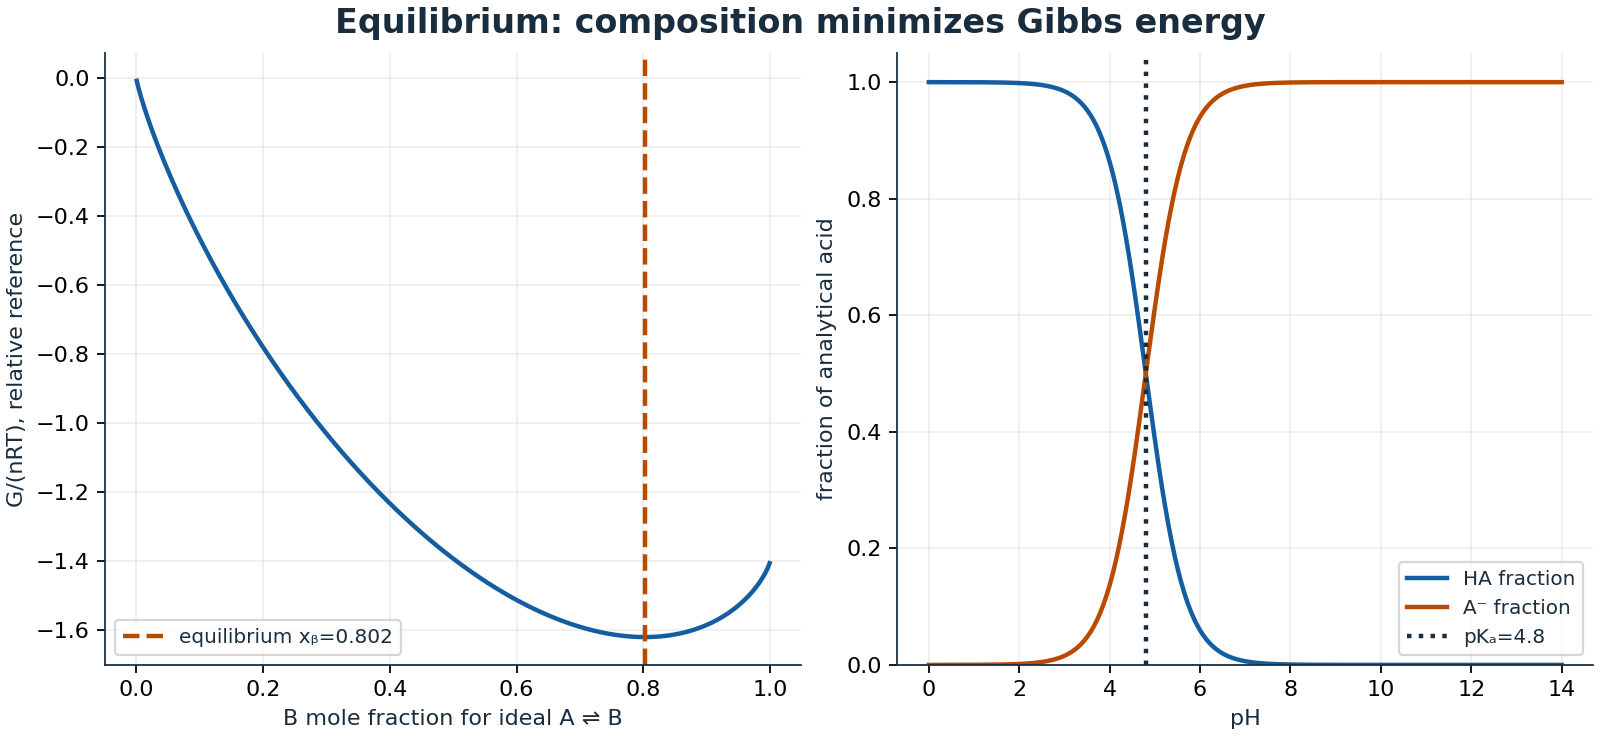
\includegraphics[width=0.95\linewidth]{tex_images/mental_map/study/chemistry_equilibrium.png}
\caption{An ideal two-species Gibbs mixing model with standard free-energy difference $-1.4RT$, and ideal acid speciation for $pK_a=4.8$. The pH curve prescribes pH; it does not independently solve a full charge-balance problem.}
\end{figure}

\subsubsection{Rates, mechanisms, and molecular explanation}
Rate laws are empirical or mechanistic statements, not usually read straight from an overall balanced equation. For a first-order disappearance, $d[A]/dt=-k[A]$, concentration decays exponentially and half-life is $\ln 2/k$. A second-order law gives different units for $k$ and a concentration-dependent half-life. Pseudo-first-order behaviour can arise when another reactant is held effectively constant; that condition must be checked.

The Arrhenius model $k=A\exp[-E_a/(RT)]$ predicts a straight line in $\ln k$ versus $1/T$ over a regime with approximately constant activation parameters. A catalyst changes the kinetic pathway and accelerates approach to equilibrium; it does not change $K$ for the same overall reaction and conditions. Curvature, diffusion limitation, or changing mechanisms can invalidate a single fitted activation energy. Reaction-coordinate energy diagrams are conceptual landscapes, not measured time trajectories.
\begin{figure}[htbp]
\centering
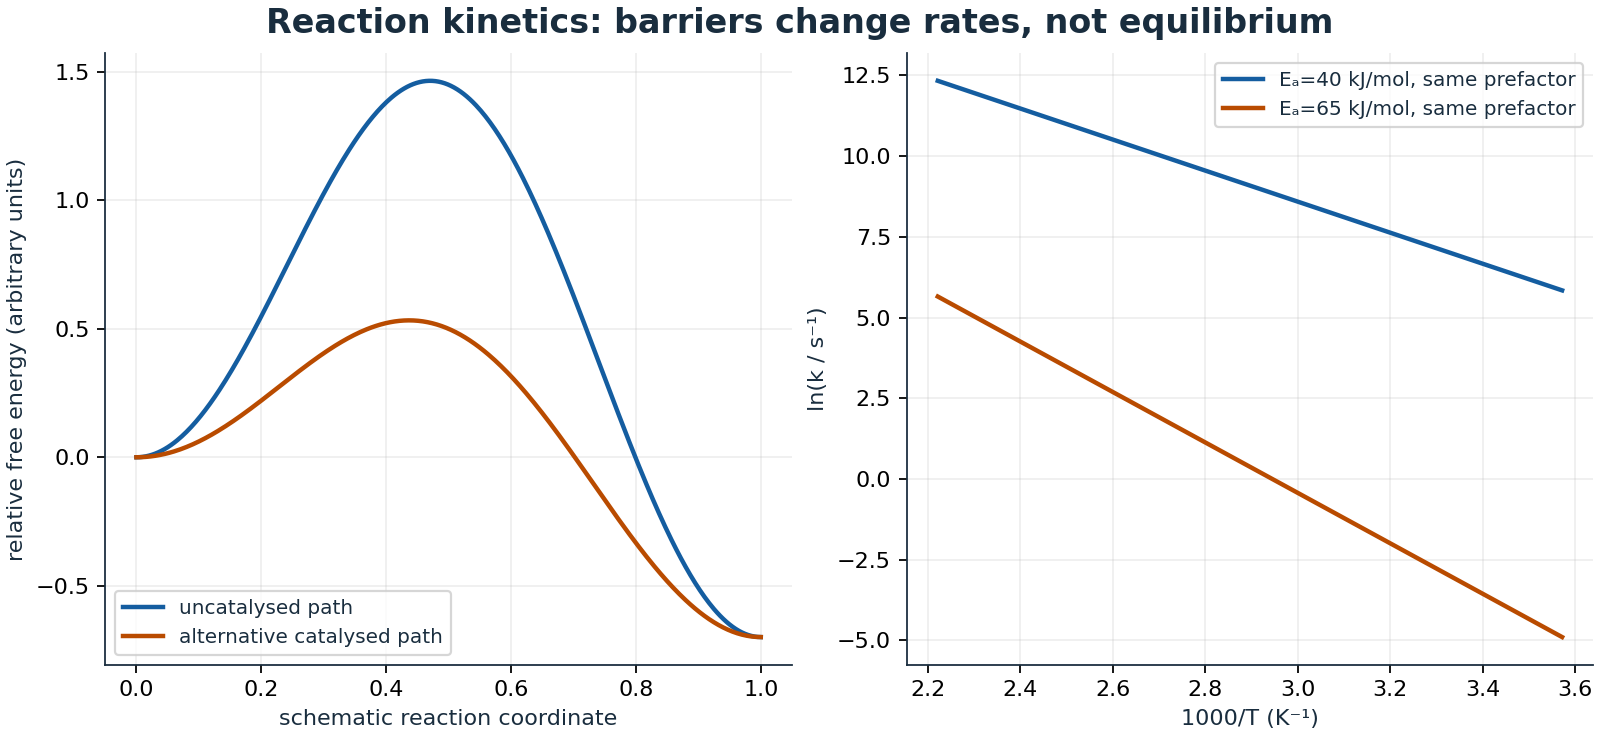
\includegraphics[width=0.95\linewidth]{tex_images/mental_map/study/chemistry_kinetics.png}
\caption{Schematic catalysed and uncatalysed paths retain identical endpoints. Synthetic Arrhenius lines assume temperature-independent prefactors and activation energies, and are not a prescription for reaction conditions.}
\end{figure}

Atomic orbitals combine into molecular orbitals; filling bonding and antibonding states explains why electron count affects bond order. For a simple two-orbital picture, bond order is $(N_b-N_a)/2$. Delocalization in conjugated systems can lower energy and change optical transitions; resonance drawings represent one electronic structure, not rapidly switching molecules. Hybridization is a useful bonding model, not a directly photographed orbital shape.

Stereochemistry distinguishes connectivity from spatial arrangement. Enantiomers are nonsuperimposable mirror images; diastereomers are stereoisomers that are not mirror partners. Conformational rotation does not generally change configuration. Mechanistic curved arrows track electron-pair movement, with charge and valence checked at each step. Concerted substitution and stepwise ionization predict different stereochemical tendencies, but solvent, substrate, competing elimination, and intermediate structure matter. Recognizing an electron-rich donor and electron-poor acceptor is more transferable than memorizing a named reaction without its assumptions.
\begin{figure}[htbp]
\centering
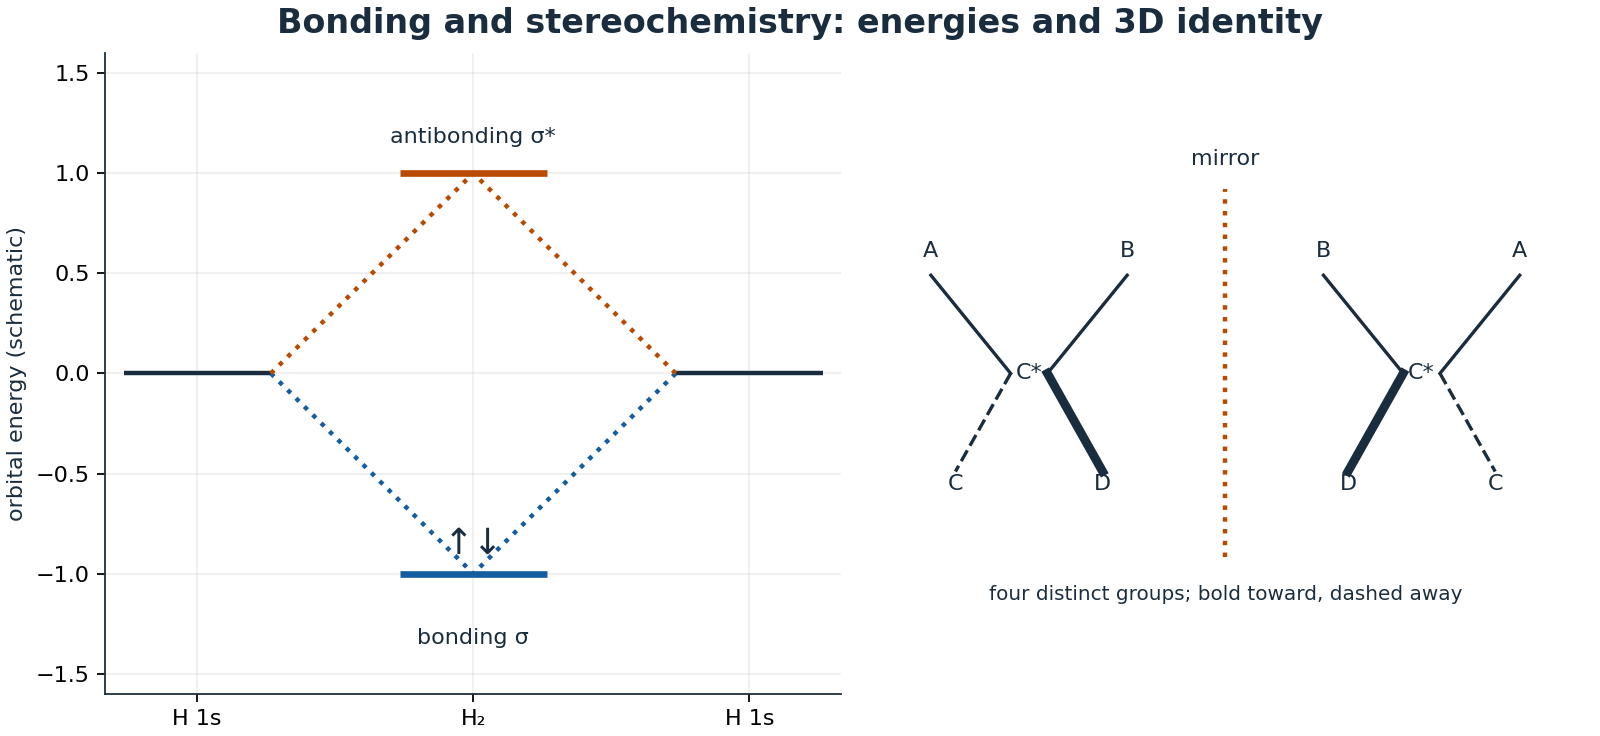
\includegraphics[width=0.95\linewidth]{tex_images/mental_map/study/chemistry_orbitals.png}
\caption{Schematic hydrogen molecular-orbital splitting and mirrored tetrahedral centres with four distinct substituents. Bold bonds point toward the viewer and dashed bonds away; no absolute configuration is assigned without priority rules.}
\end{figure}

\subsubsection{Polymers and biochemical function}
Polymer properties depend on chain length distribution, branching, tacticity, crystallinity, cross-linking, and temperature. Number-average and mass-average molar masses differ:
\begin{equation}
M_n=\frac{\sum_iN_iM_i}{\sum_iN_i},\qquad
M_w=\frac{\sum_iN_iM_i^2}{\sum_iN_iM_i},\qquad
D=M_w/M_n\geq1.
\end{equation}
Step-growth and chain-growth describe different growth mechanisms, not simply slow versus fast reactions. Glass transition marks a change in segmental mobility; melting concerns crystalline order. Cross-linked networks can exhibit elastic recovery while lacking ordinary melt flow. Mechanical behaviour therefore cannot be inferred from chemical repeat-unit identity alone.

Proteins combine amino-acid chemistry with folding, electrostatics, and solvent interactions. Lipids organize interfaces, carbohydrates store energy and encode recognition, and nucleic acids carry sequence information. Enzyme catalysis depends on structure and environment. The Michaelis--Menten initial-rate model $v=V_{\max}[S]/(K_m+[S])$ assumes a suitable simple mechanism, approximately steady intermediate concentration, and negligible product effects. $K_m$ is not universally a binding dissociation constant. Denaturation, inhibition, transport, and substrate depletion can all make a fitted saturation curve misleading.
\begin{figure}[htbp]
\centering
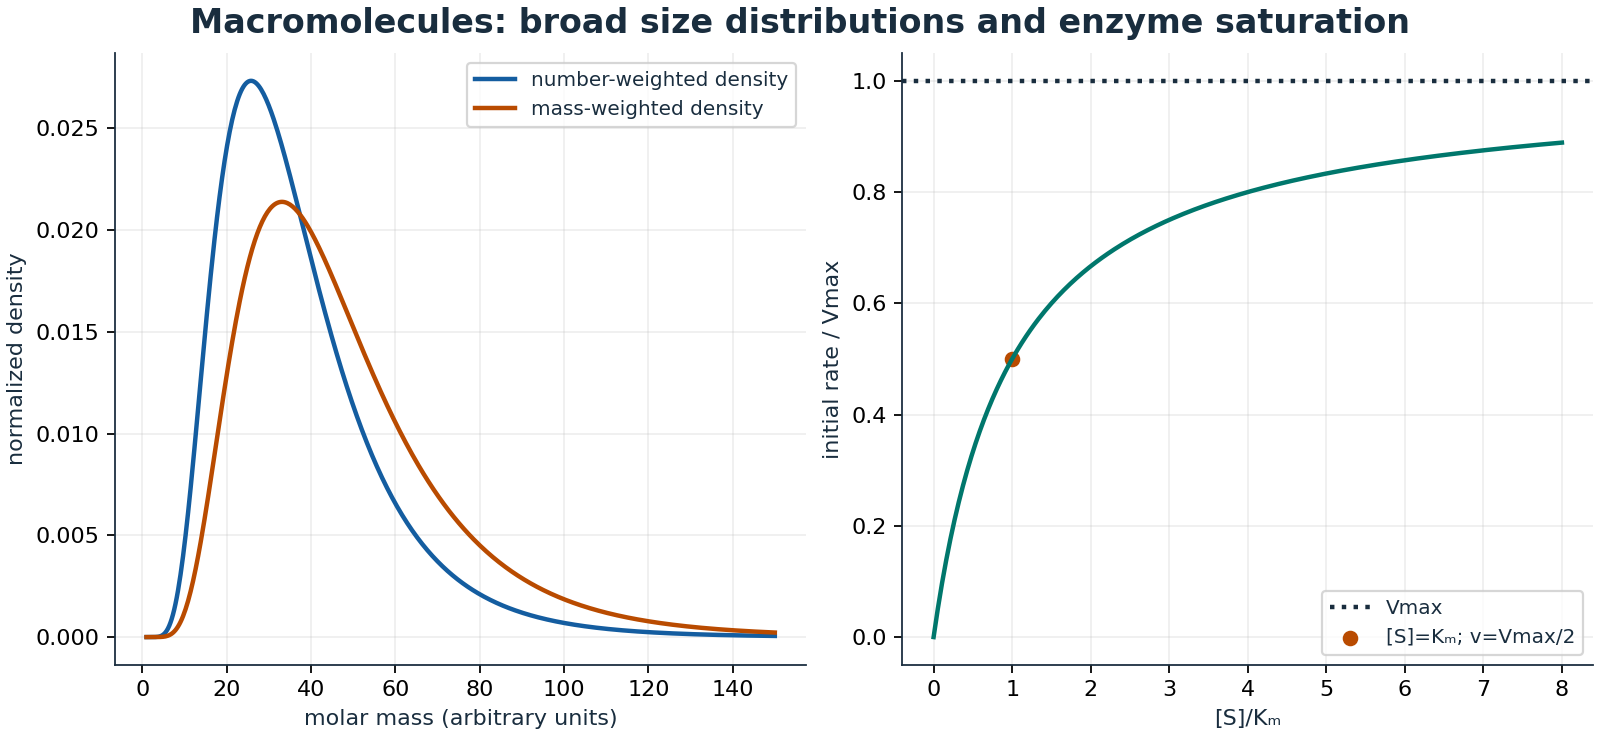
\includegraphics[width=0.95\linewidth]{tex_images/mental_map/study/chemistry_polymers.png}
\caption{A synthetic broad molar-mass distribution weighted by molecule count or mass, and ideal enzyme-rate saturation. Neither curve represents a particular polymer batch or biological assay.}
\end{figure}

\subsubsection{Characterization, uncertainty, and safety}
FTIR probes vibrational modes that change dipole moment; Raman probes changes in polarizability. Their selection rules are complementary, not interchangeable peak catalogues. X-ray diffraction relates ordered spacings to $2d\sin\theta=n\lambda$; peak broadening may reflect domain size, strain, or instrumental effects. SEM contrast depends on electron interactions, detector, charging, and sample geometry. AFM measures a tip--surface interaction through a feedback system, with finite tip geometry broadening narrow lateral features.
\begin{figure}[htbp]
\centering
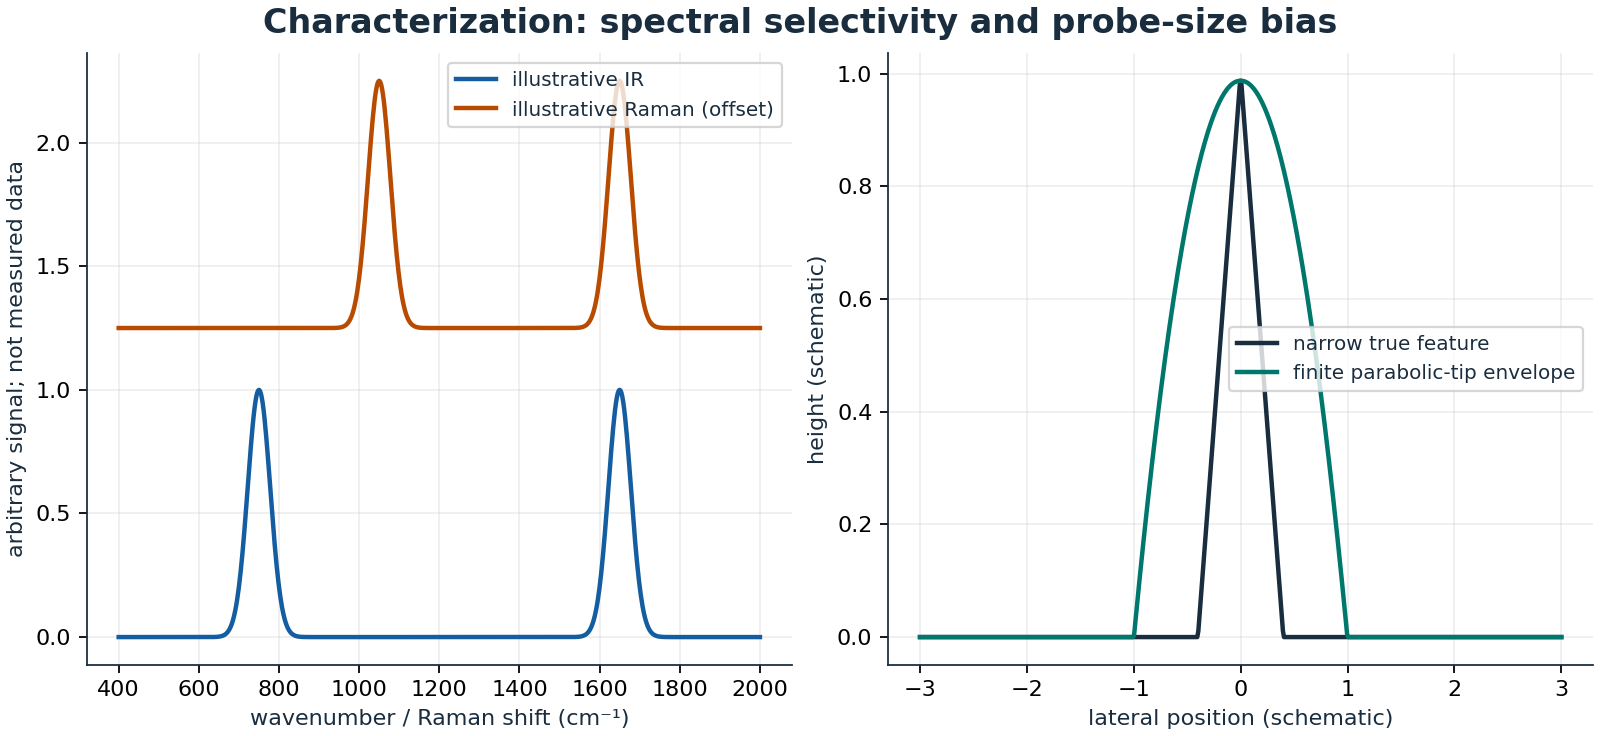
\includegraphics[width=0.95\linewidth]{tex_images/mental_map/study/chemistry_characterization.png}
\caption{Invented IR and Raman signals illustrate differing selection rules, without assigning real chemical peaks. A parabolic-tip envelope demonstrates AFM lateral broadening; real feedback and mechanical artefacts add further uncertainty.}
\end{figure}

Use standards, blanks, repeat measurements, calibration, and complementary techniques. Distinguish instrument resolution from accuracy and detection limit from quantified concentration. Propagate uncertainty as in Section~\ref{study-math}; a visually sharp peak is not proof of a unique phase or composition. Nanomaterial hazards depend on size, shape, exposure route, persistence, and surface chemistry. Consult institutional procedures and safety data, use trained supervision and appropriate containment, and assess waste handling. These notes deliberately omit operating recipes and do not authorize unsupervised chemical work.

\subsubsection{Sources and scope}
The \href{https://ucalendar.uwaterloo.ca/2223/COURSE/course-NE.html}{Waterloo 2022/23 NE calendar} motivates the chemical principles, organic chemistry, biochemistry, materials characterization, and macromolecular themes. See \href{https://openstax.org/details/books/chemistry-2e}{OpenStax Chemistry 2e} for foundational balance, equilibrium, kinetics, and bonding. Calendar listings, including later-introduced courses, are scope references only and do not establish a personal study history.